We were required to write report in style of a technical paper so that it could be ultimately submitted to a conference/journal. Also the team was required to write the report collectively, hence overleaf account with document sharing feature helped.\\
We used overleaf account to build the report using LaTeX due to ease of access and modularization.\\
Reasons to opt for latex over other documenting tools:
\begin{itemize}
    \item[$-$] Open source technology
    \item[$-$] Provides professional output
    \item[$-$] Highly flexible structure and huge number of formatting options
    \item[$-$] Sections can be easily modularized
    \item[$-$] Easy to maintain, for ex can be could be integrated with GitHub
    \item[$-$] Allows access from multiple people to work independently on report
    \item[$-$] Easy to manage image and code references
\end{itemize}

\begin{figure}[H]
    \centering
    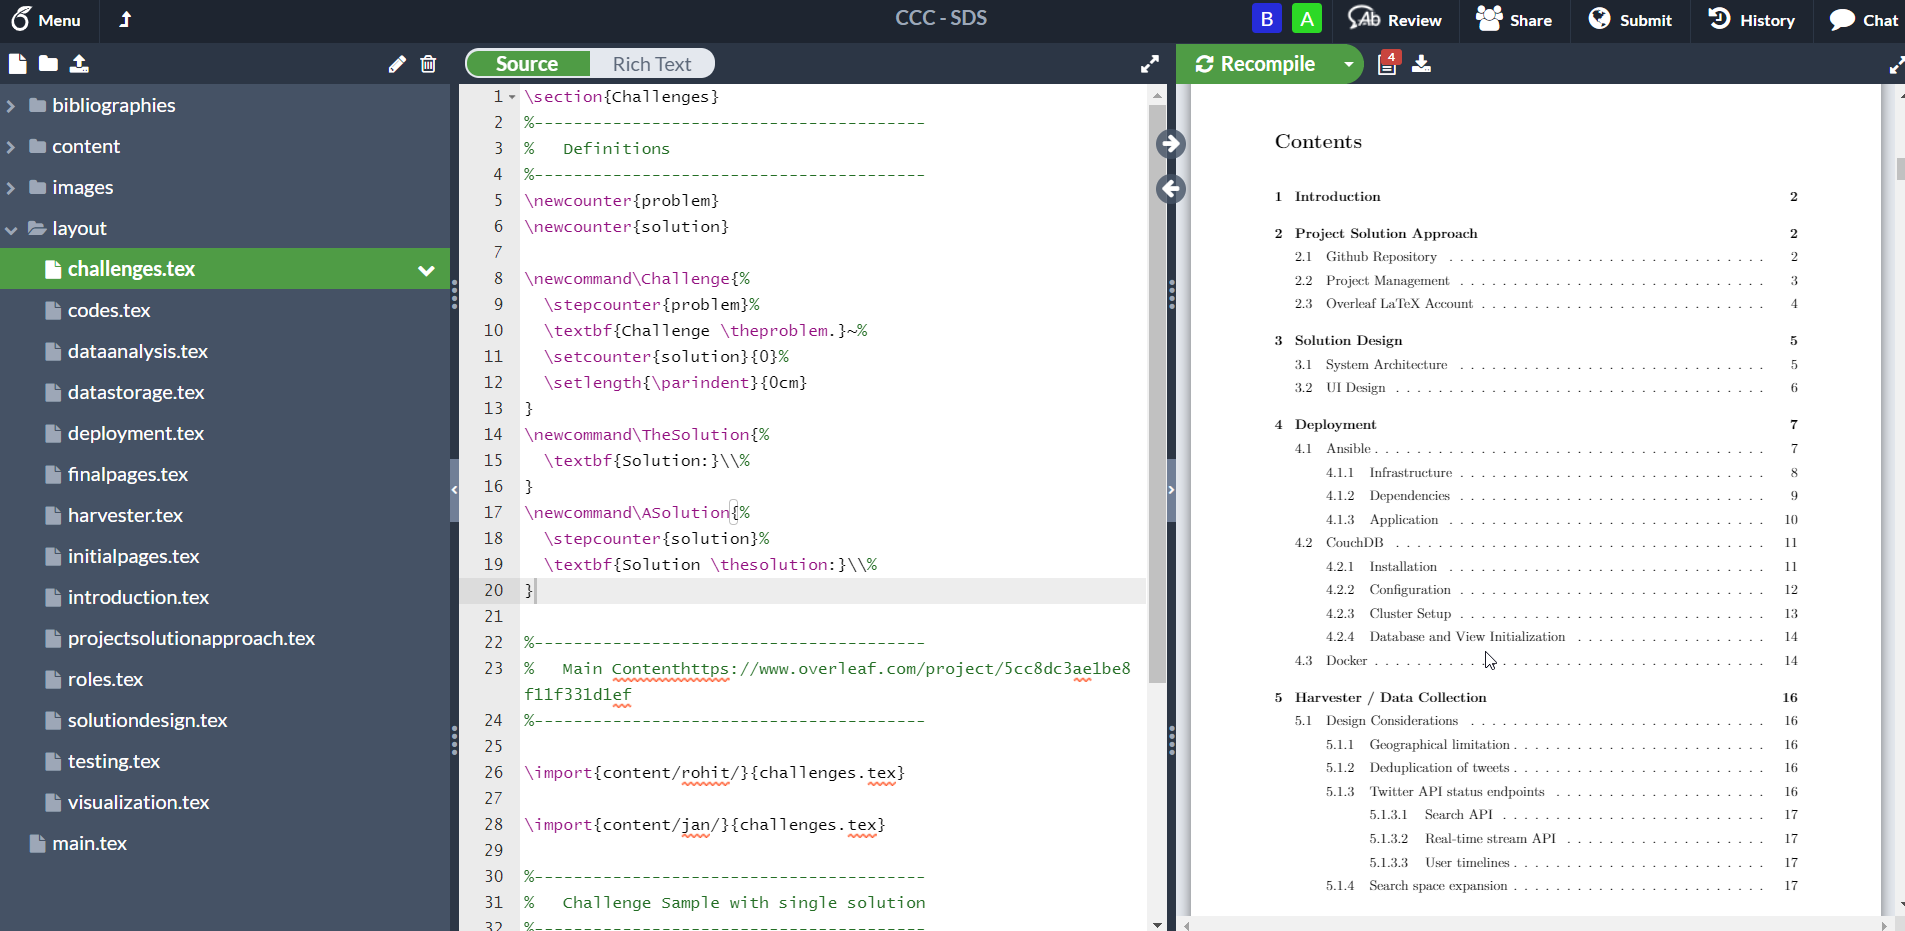
\includegraphics[width=14cm,keepaspectratio=true]{images/latex/latex_overview1.png}
    \caption{LaTeX Overview - Overall Structure}
    \label{fig:latex_overview1}
\end{figure}

\begin{figure}[H]
    \centering
    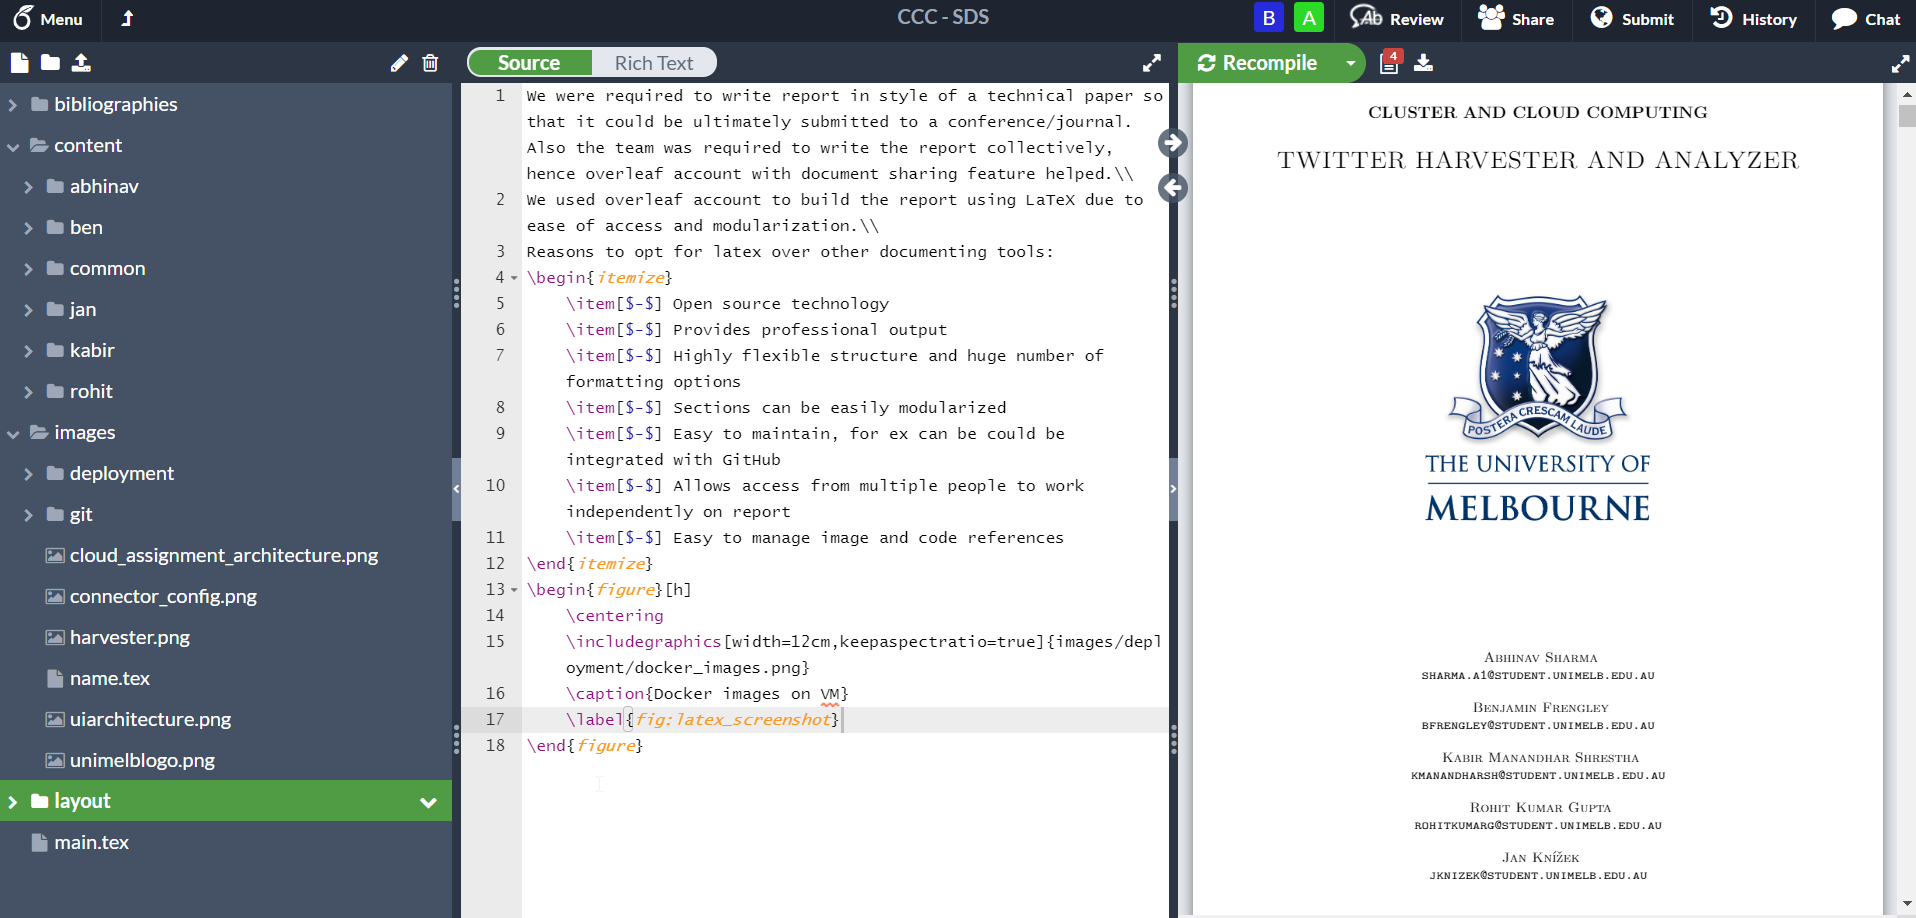
\includegraphics[width=14cm,keepaspectratio=true]{images/latex/latex_overview2.png}
    \caption{LaTeX Overview - Individual Modules}
    \label{fig:latex_overview2}
\end{figure}